\section{Hardware review: suggested, thesis, built}

This section is my review of the hardware as I found it in September 2026, compared with what Stanford
suggests and what the thesis describes. Where the three disagree, the lab hardware is what counts; every
difference below was checked on the towers, with the photo or measurement named in the repository.

\subsection{Comparison}

{\small
\begin{longtable}{>{\raggedright}p{2.6cm} >{\raggedright}p{3.9cm} >{\raggedright}p{3.6cm} >{\raggedright\arraybackslash}p{4.6cm}}
\toprule
Function & Stanford suggests (BOM, guide) & Thesis (2026) & Built and checked (Oct 2026) \\
\midrule\endhead
\bottomrule\endfoot
Controller & Speedgoat real-time target, 1000\,Hz; Teensy named as an untested option & Teensy 4.1 + Adafruit MCP4728 DAC on a breadboard, 10\,ms loop & Same parts. Firmware rewritten (v1, fixed-rate 10\,ms). Breadboard being replaced by a carrier PCB (Sect.~\ref{sec:carrier}) \\
Motor & maxon EC 90 flat 500267 (260\,W, 48\,V, Hall) & same & same on all four towers (labels read) \\
Motor driver & maxon ESCON 70/10 (422969) & same & same; tower B's is faulty, replacement ordered \\
Brake chopper & maxon DSR 70/30 (235811), threshold 55\,V & same, threshold not stated & same; three at 55\,V, tower B was at 75\,V (all DIP switches off), set to 55\,V \\
48\,V supply & Mean Well RSP-2000-48, one per module & same & same; tower B's old supply faulty (white residue), replaced \\
Force sensor & Strain-gauge ``dogbone'' (Omega SGD-7/1000) with a home-made bridge board, optional & DYMH-103 S-type load cell, 100\,kg & DYMH-103 100\,kg, 1.6\,mV/V; one amplifier found paired with a 200\,kg, 1.0\,mV/V cell \\
Amplifier & Futek IAA100 & Futek IAA100, trimmed 0--3.3\,V = 0--200\,N & same \\
24\,V supply & small 24\,V adapter per amplifier & Mean Well RS-15-24 per amplifier & same; printed mounting plates designed \\
Encoder & Renishaw RM22, optional & not used & not used \\
Frame & 80/20 inch profiles (1020, 2020) & ``80$\times$80\,mm'' profiles & 90$\times$90 light, B-type (Bosch-compatible), slot 10; parts held by M6 ISO~7380 button heads in slot-10 T-nuts \\
Signal cable & igus chainflex CF240, 7 cores & lab multi-core cable spliced to jumper wires & same cable, jumpers replaced by one colour per signal, ends going into pluggable connectors \\
Chopper $\rightarrow$ ESCON & 14\,AWG, 2-core & not stated & 14\,AWG is too thick for the chopper terminals (max 1.5\,mm$^2$): use pin terminals (Sect.~\ref{sec:power}) \\
E-stop & e-stop button, one NO contact per 48\,V supply on CN501 & treadmill e-stop only & not wired yet; parts listed (Sect.~\ref{sec:estop}) \\
Control law & feedforward gain 1, 60\,Hz Butterworth filter, 3-sample derivative, separate gain sets & feedforward 7.5, no filter, 1-sample derivative & thesis values are the firmware defaults; every value is now a runtime parameter (Sect.~\ref{sec:firmware}) \\
\end{longtable}
}

\subsection{Notes per component}

\paragraph{Motor.} All towers carry the maxon EC 90 flat, part 500267 (11 pole pairs, torque constant
231\,mNm/A, terminal resistance 0.844\,$\Omega$). The firmware still uses $k_t = 0.1524$, a value from the
original code whose origin is unknown. Changing it changes the force produced per command; decide together
with \cmd{i\_full} (below) after the closed-loop tests.

\paragraph{ESCON setpoint scaling.} The ESCON maps its analog input 0--10\,V to 0--30\,A (read from module
A's driver, \file{escon/moduleA_left_2026-10-01.edc}). The DAC only reaches 3.3\,V, so its full scale is
\textbf{9.9\,A}, while the firmware parameter \cmd{i\_full} assumes 30\,A. The thesis peak forces
(82--115\,N at a 100\,N target) are consistent with this 9.9\,A ceiling. Do not change \cmd{i\_full} or the
ESCON scaling before reading every driver's configuration: the commanded current would rise about three times.

\paragraph{Brake chopper threshold.} The chopper burns the energy the motor feeds back when it brakes. Its DIP
switches set the threshold: $V_\mathrm{th} = 75\,\mathrm{V} - (\text{sum of switches ON}) \times 1\,\mathrm{V}$
(S1 = 1, S2 = 2, S3 = 4, S4 = 8, S5 = 16, S6 = 32). Stanford uses 55\,V (S3 + S5 ON). ``ON'' is printed on the
side opposite the numbers. The broken tower had all switches OFF (75\,V), above the ESCON's 70\,V maximum and
the supply's over-voltage limit: a plausible cause of the old failure, not proven.

\paragraph{Force sensing.} Each module: DYMH-103 load cell in the rope $\rightarrow$ Futek IAA100 amplifier
$\rightarrow$ Teensy analog input (10 bit, so 200\,N/1023 $\approx$ 0.2\,N per count). The thesis
calibrated four sensors with 6, 8 and 12\,kg (error below 2.5\,\%). Which sensor sits on which tower is not
recorded; recalibrate per module after the carrier board. A fourth amplifier was found with a 200\,kg,
1.0\,mV/V cell: about three times less signal per newton, so check it with weights before use.

\paragraph{Frame.} The thesis value of 80$\times$80\,mm is outdated. The towers are 90$\times$90 light B-type
profiles with 10\,mm slots (e.g.\ Motedis ``Aluprofil 90x90 L B-Typ Nut 10''), not item and not the heavy
Rotec profile. This matters for anything you mount: use slot-10 T-nuts.

\paragraph{Ground distributor.} Each tower has a small board in the frame that joins ESCON J5 pin 5, ESCON
J6 pin 7 and the IAA100 ground; one wire per tower goes from it to the Teensy ground. The manual calls it the
``Distributor''.

\begin{figure}[H]\centering
\begin{minipage}{0.32\linewidth}\centering
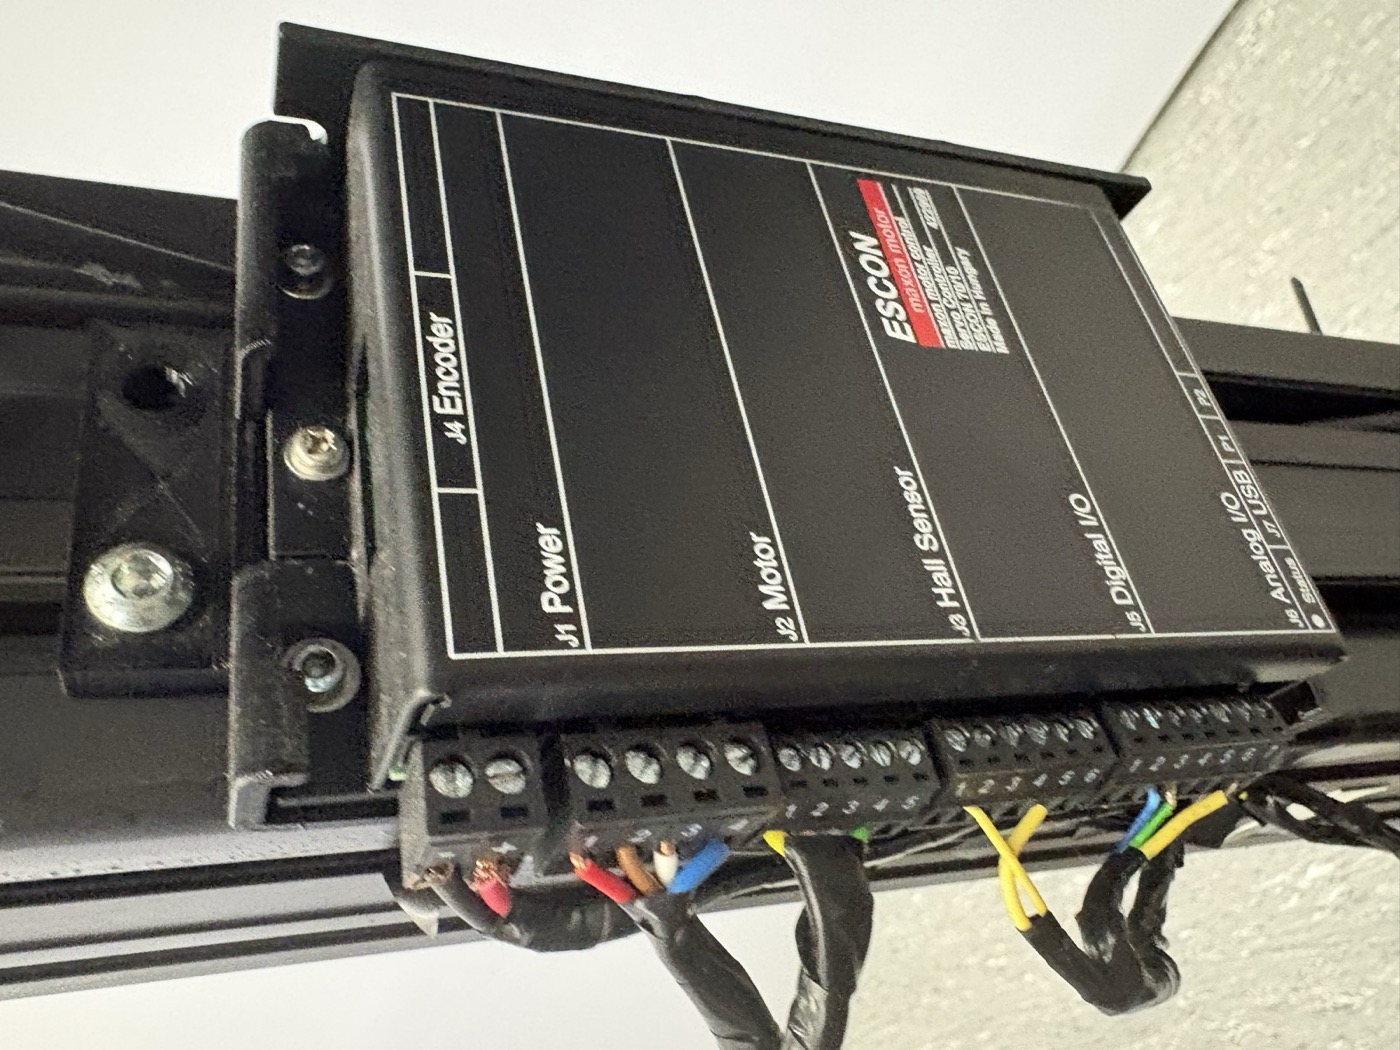
\includegraphics[width=\linewidth]{figures/2026-09-29_escon-7010-connectors.jpg}\\\small ESCON 70/10, terminal side
\end{minipage}\hfill
\begin{minipage}{0.32\linewidth}\centering
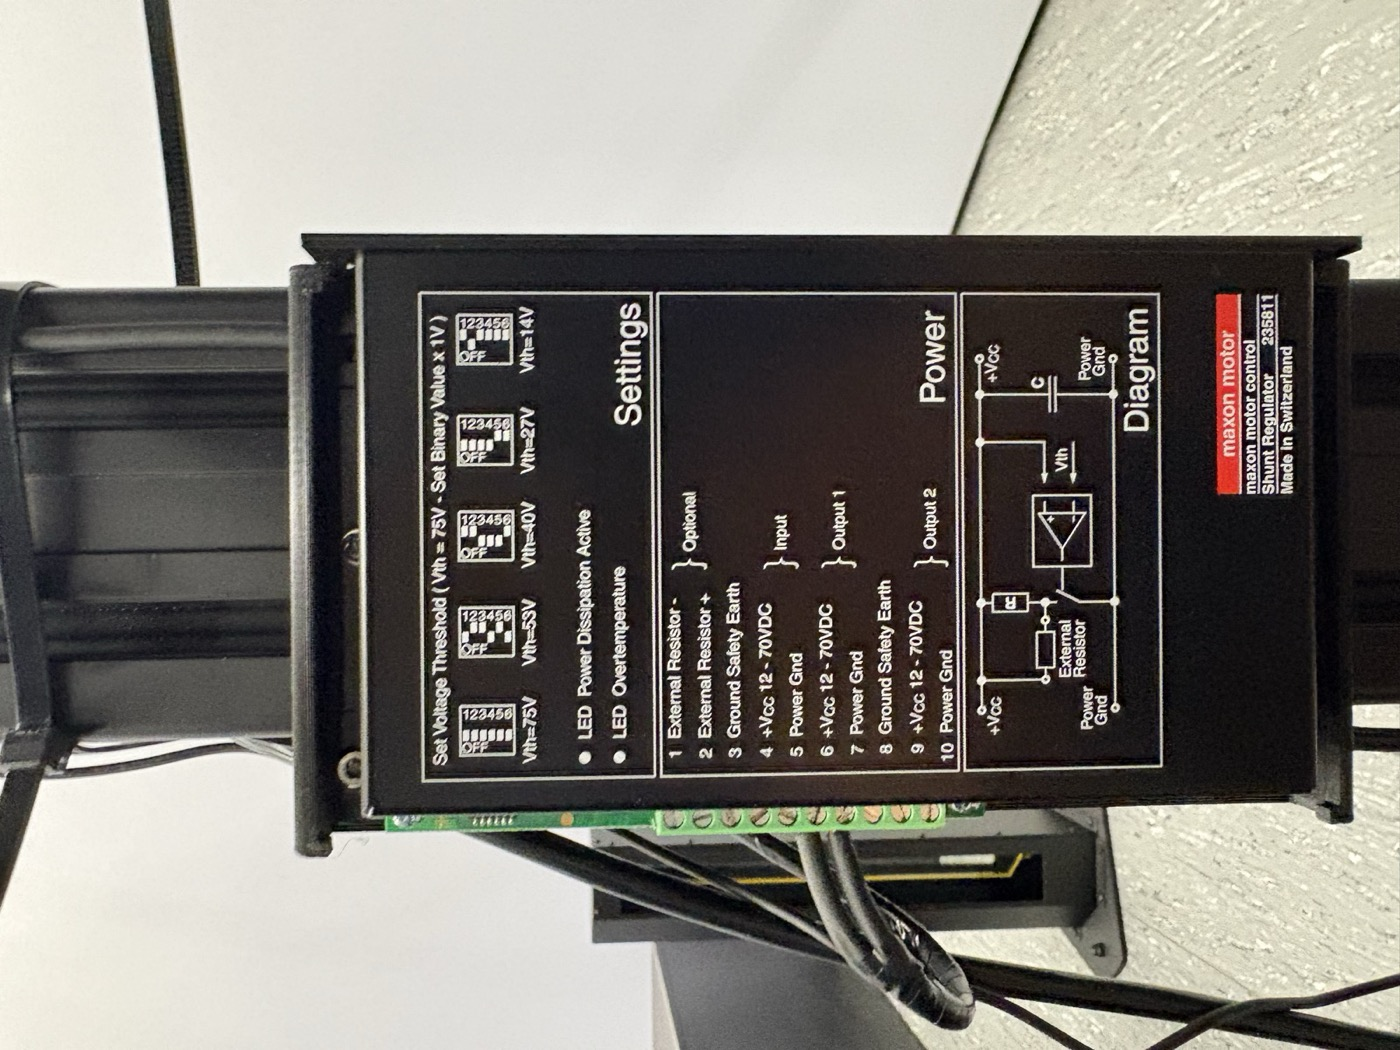
\includegraphics[width=\linewidth]{figures/2026-09-30_shunt-regulator.jpg}\\\small Brake chopper DSR 70/30
\end{minipage}\hfill
\begin{minipage}{0.32\linewidth}\centering
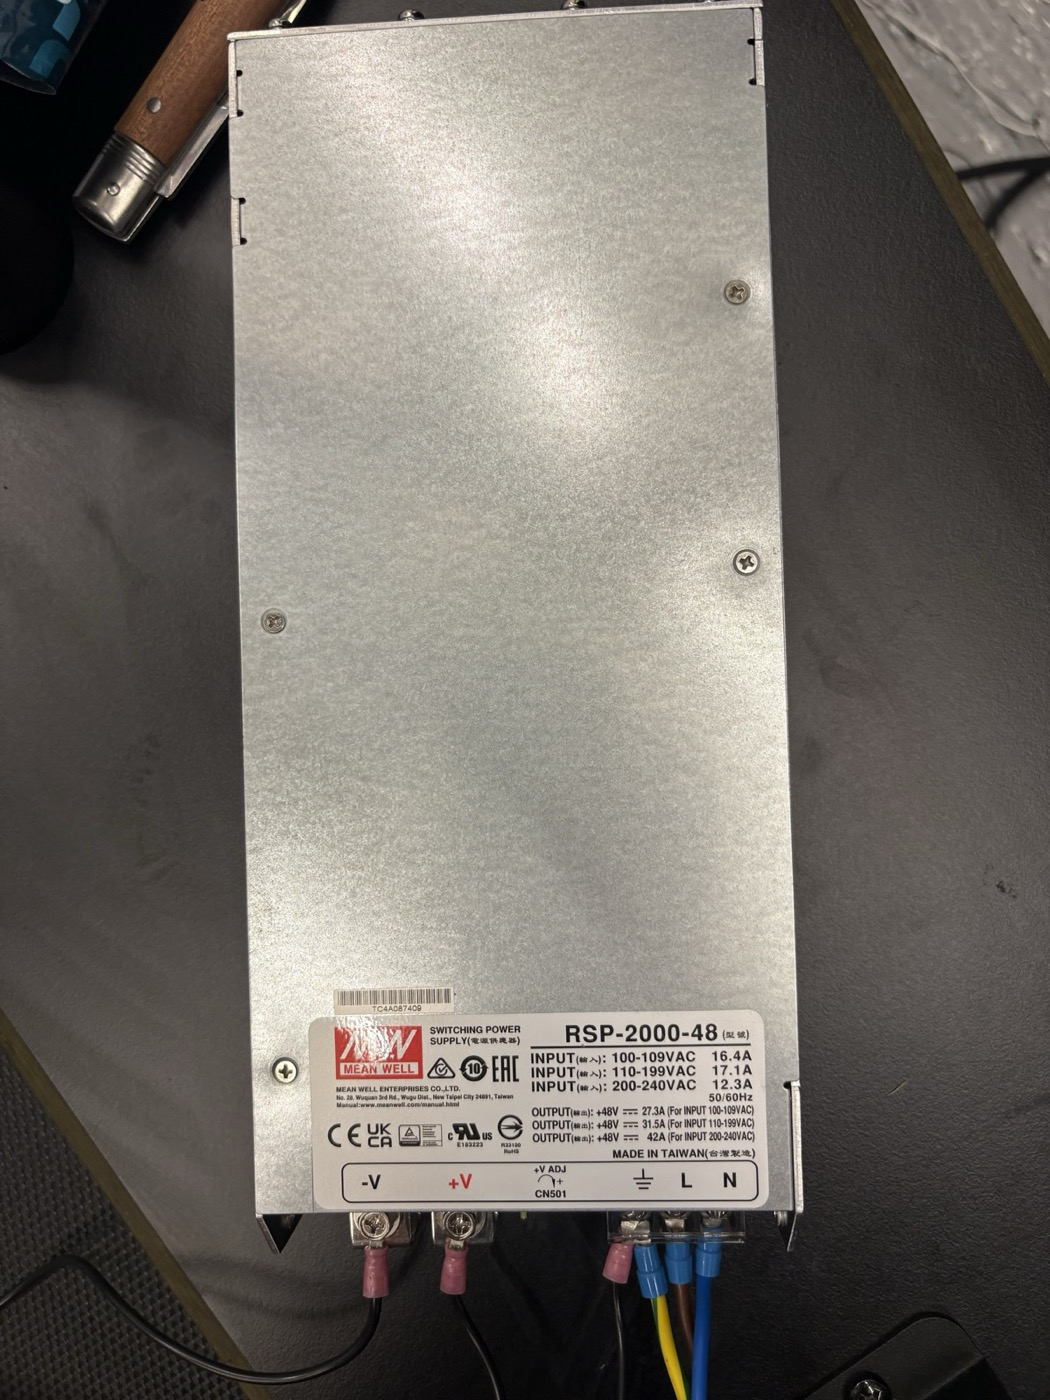
\includegraphics[width=\linewidth]{figures/2026-09-30_48V-psu-meanwell-rsp-2000-48.jpg}\\\small 48\,V supply RSP-2000-48
\end{minipage}
\caption{Per-tower power electronics (photos 29--30 Sep 2026).}
\end{figure}

\subsection{Material bought and to buy}
Prices are from the order or the shop page on the date given; check before ordering again.
Full lists: \file{docs/parts-list.xlsx} (one complete tower), \file{docs/parts-to-buy.xlsx}.

{\small
\begin{longtable}{>{\raggedright}p{4.2cm} >{\raggedright}p{4.0cm} >{\raggedright}p{2.2cm} >{\raggedright\arraybackslash}p{4.3cm}}
\toprule
Item & Part & Status & Why / note \\
\midrule\endhead
\bottomrule\endfoot
Motor driver, tower B & maxon ESCON 70/10, 422969 & ordered 7 Oct 2026 & old one: enable and USB dead. maxongroup.de, EUR 417.67 + EUR 14.90 shipping + VAT = EUR 514.76 \\
48\,V supply, tower B & Mean Well RSP-2000-48 & in use & old one faulty. \fillin{source / order} \\
Carrier PCB & \file{hardware/carrier/fab} & being made & HS Offenburg makerspace, bare copper, expected 16 Oct 2026 \\
Carrier parts & 2$\times$ female header 1$\times$24, 2$\times$ 1$\times$6; 4$\times$ Phoenix MSTB 2,5/5-GF-5,08 (1776537) + 4$\times$ plug MSTB 2,5/5-STF-5,08 (1778014); 4$\times$ 1\,k$\Omega$, 4$\times$ 1\,M$\Omega$, 4$\times$ BAT85 & to buy / makerspace & BOM \file{hardware/carrier/fab/bumpem-carrier-bom.csv} \\
Ferrules 0.25--0.5\,mm$^2$ & & to buy & 5 signal wires per module plug; never tin wire tips under a screw \\
Pin terminals, blue, 1.5--2.5\,mm$^2$ + crimper for insulated terminals & & to buy & 14\,AWG chopper $\rightarrow$ ESCON cable, tower B \\
Screws & M3$\times$6, M4$\times$12, M6$\times$16 ISO~7380, slot-10 T-nuts & to buy & printed parts (Sect.~\ref{sec:printed}); M6 length to confirm on the test print \\
E-stop & Hirose DF11-12DS housing + DF11 crimp terminals per 48\,V supply; button with one NO contact block per supply & to order & Sect.~\ref{sec:estop} \\
Load cell (spare) & DYMH-103, 100\,kg & only if needed & if the 200\,kg cell fails calibration \\
Brake chopper (spare) & maxon DSR 70/30, 235811 & not needed & tower B's chopper passed at 24\,V and 48\,V \\
\end{longtable}
}

Not bought, already in stock: motors, choppers (4), RSP-2000-48 (3 + B's), RS-15-24 (4), IAA100 (4),
load cells, Teensy 4.1, MCP4728, frame.

\subsection{Printed tower parts}\label{sec:printed}
To get the electronics off the floor and off tape, I designed printed holders that bolt into the profile
slots (\file{hardware/enclosures/}, CadQuery; overview \file{hardware/enclosures/out/parts-overview.pdf}).
All slot and bolt dimensions live in \file{tower.py}; device sizes come from the datasheets in
\file{docs/reference/}.

\begin{figure}[H]\centering
\begin{minipage}{0.24\linewidth}\centering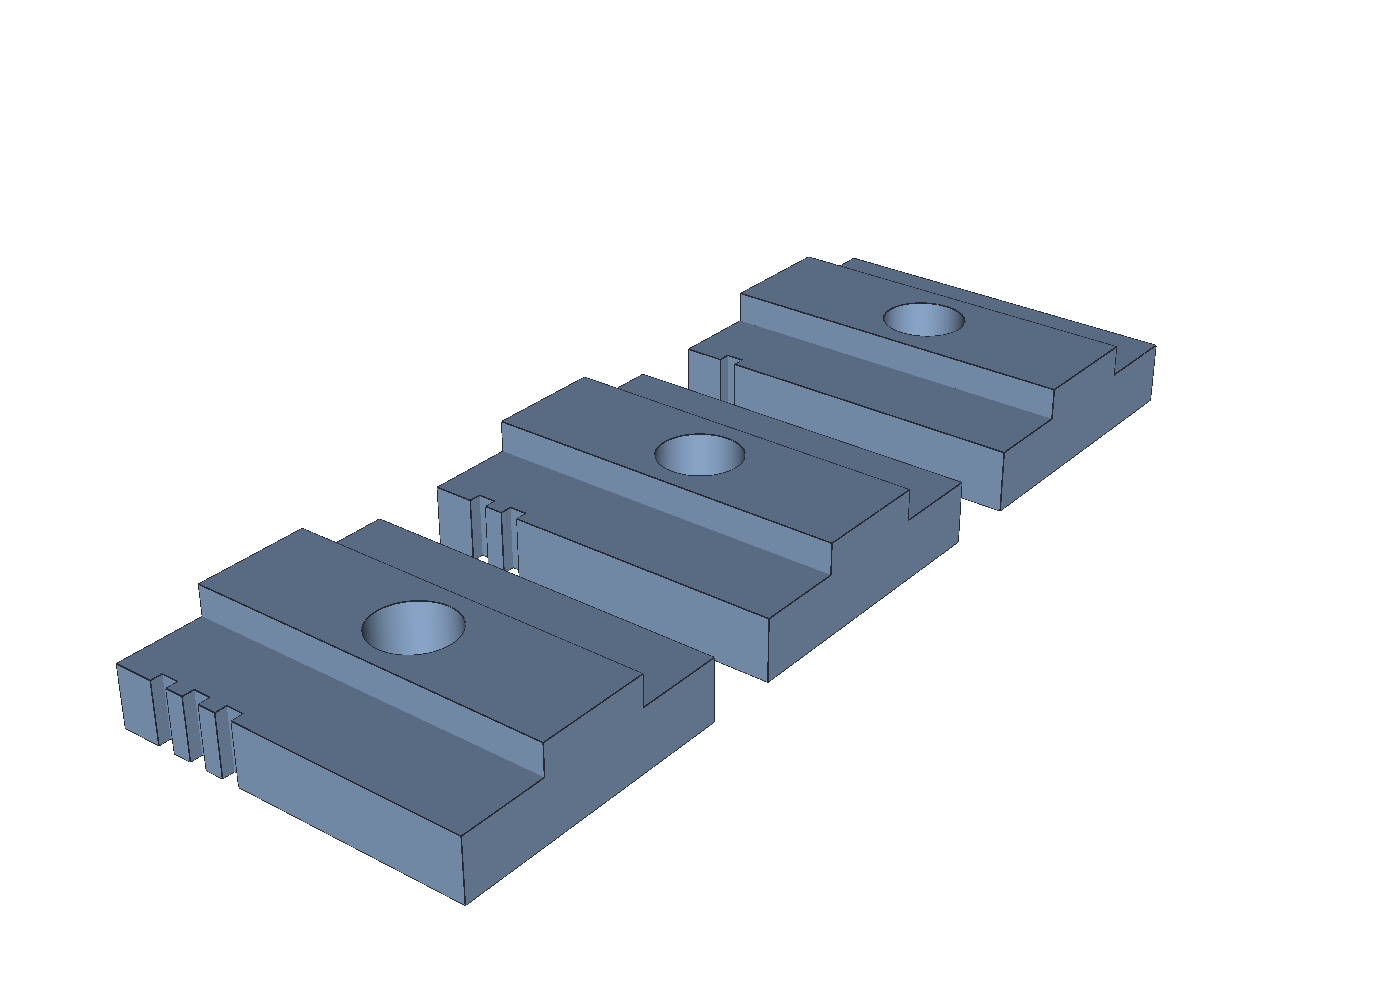
\includegraphics[width=\linewidth]{figures/render-testplates.png}\\\scriptsize slot test plates (0.1/0.2/0.3\,mm)\end{minipage}\hfill
\begin{minipage}{0.24\linewidth}\centering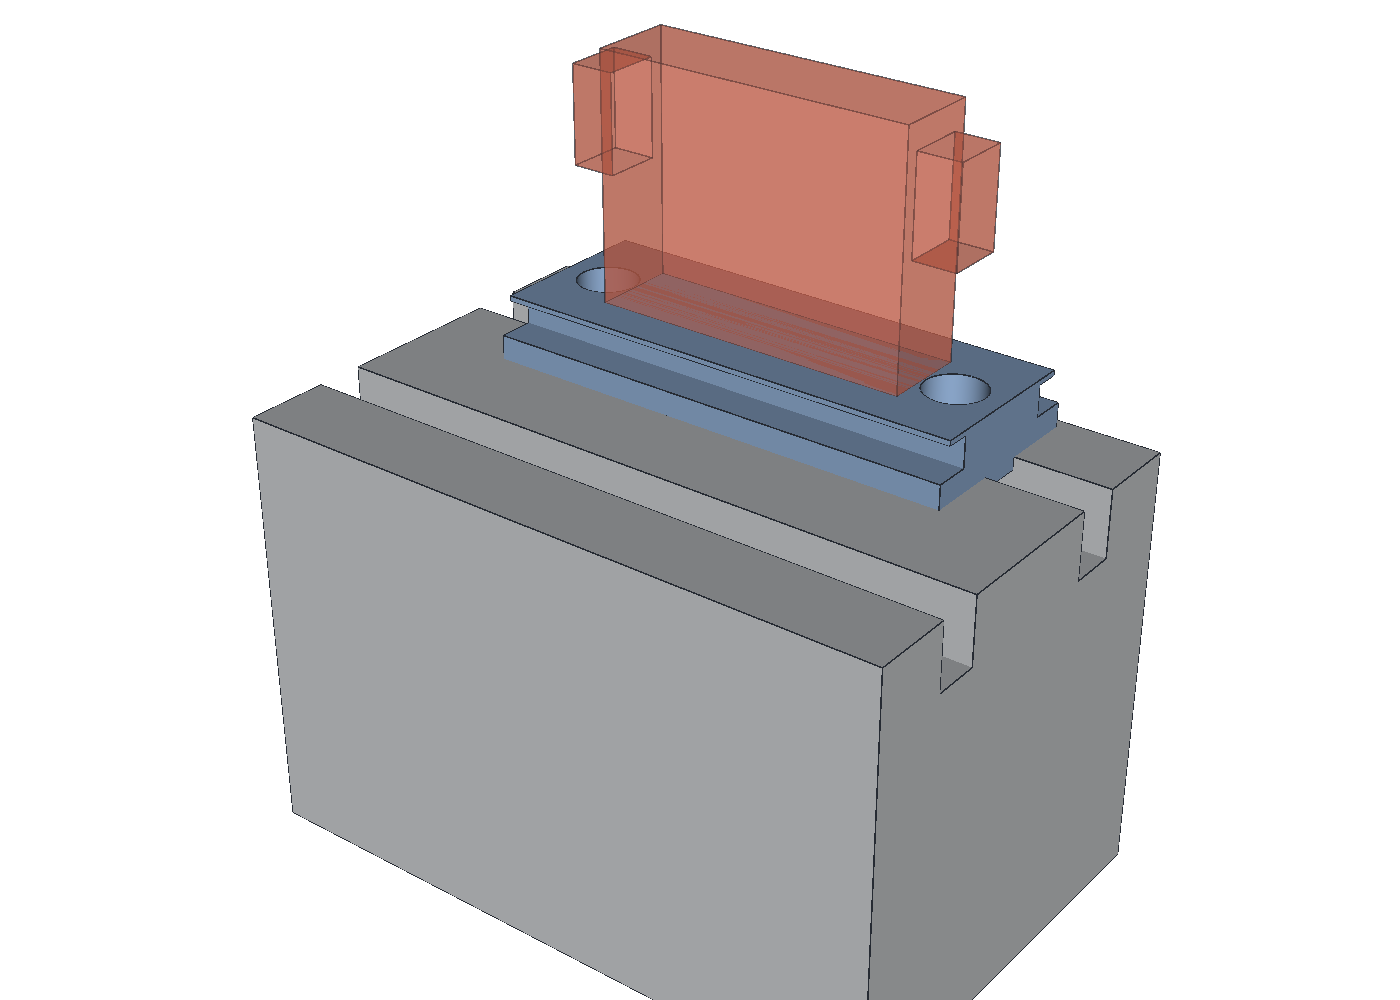
\includegraphics[width=\linewidth]{figures/render-iaa100.png}\\\scriptsize IAA100 on a printed DIN rail\end{minipage}\hfill
\begin{minipage}{0.24\linewidth}\centering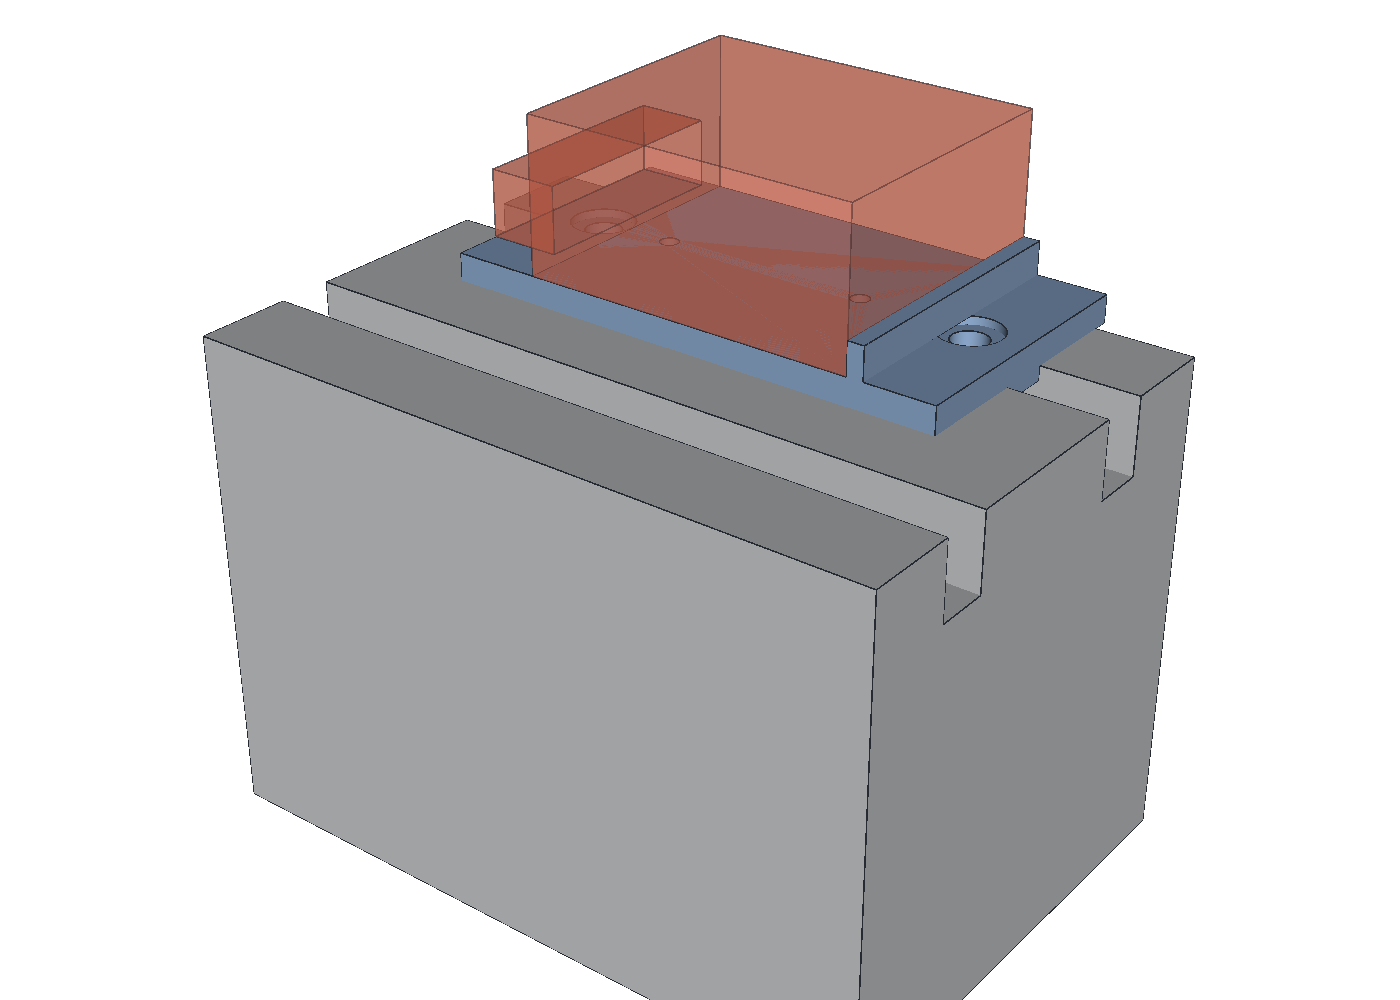
\includegraphics[width=\linewidth]{figures/render-rs15.png}\\\scriptsize RS-15-24 plate, 2$\times$M3$\times$6\end{minipage}\hfill
\begin{minipage}{0.24\linewidth}\centering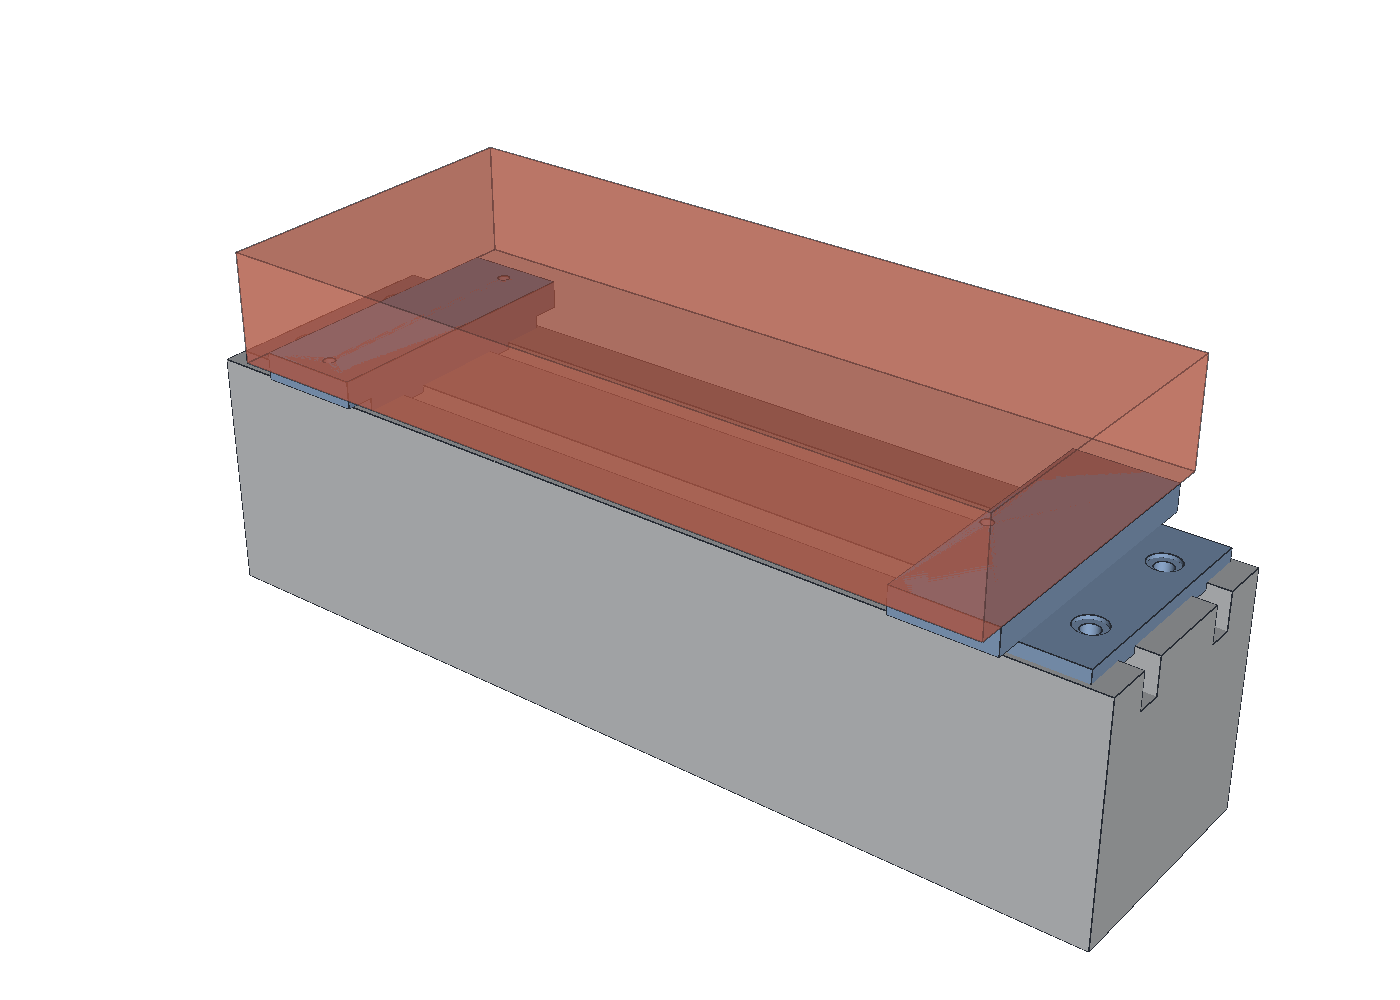
\includegraphics[width=\linewidth]{figures/render-rsp2000.png}\\\scriptsize RSP-2000 brackets, M4$\times$12, 10\,mm air gap\end{minipage}
\caption{Printed parts. Print PETG or ASA (48\,V brackets: ASA, or PETG $\geq$ 40\,\% infill).}
\end{figure}

To change a part: edit \file{tower.py} or \file{parts.py}, then run \cmd{python make\_stl.py} and
\cmd{python overview.py} in that folder (needs \cmd{pip install cadquery matplotlib vtk}). After the test
print, set \cmd{KEY\_CLEAR} in \file{tower.py} to the plate that slid in without play (currently 0.2\,mm).
